\begin{center}
	\hrule
	\vspace{.4cm}
	{\textbf { \large ELEC 460 --- Control Theory II}}
\end{center}
{\textbf{Name:}\ David Li \hspace{\fill} \textbf{Student Number:}} \ V00818631  \\
{\textbf{Due Date:} Friday, 26 January 2018, 11:30 AM \hspace{\fill} \textbf{Assignment:} Number 2 \\
	\hrule
	
% Questions are taken from the textbook
\paragraph{B-2-7}
%\vspace{-1cm}
%Obtain the z-transform of the curve.

%\[
%f(x)=
%\begin{cases}
%& x < 2  = 0\\
%& 2 \geq x \leq 5 = \frac{x-2}{3} \\
%& x \geq 5 = 1
%\end{cases}
%\]
% \vspace{-1cm}
%\begin{figure}[H]
%	\centering
%	\resizebox{\textwidth}{!}{%
%	\begin{tikzpicture}[
%	declare function={
%		func(\x)= (\x < 2) * (0)   +
%		and(x >= 2,\x<=5) * ((\x-2)/3)     +
%		(\x>5) * (1)
%		;
%	}, 
%	]
%	\begin{axis}[
%	axis x line=middle, axis y line=middle,
%	ymin=0, ymax=1, ytick={0,0.25,0.5,0.75,1.0}, ylabel=$x(t)$,
%	xmin=0, xmax=8, xtick={-1,...,8}, xlabel=$t$,
%	domain=-0:8,samples=101, % added
%	]
%	
%	\addplot [blue,thick] {func(x)};
%	%\addplot[mark=none, black, samples=2] {1};
%    \addplot[black,line join=round,dashed] coordinates { (0,1) (5,1) };
%	\addplot[gray,line join=round,dashed] coordinates { (5,0) (5,1) };
%	% Also see https://tex.stackexchange.com/questions/399750/plot-dash-lines-on-plot-specifying-coordinates/399764
%	\end{axis}
%	\end{tikzpicture}}
%\end{figure}

%The function can be expressing using the heaviside $u(t)$.
%\begin{align*}
%& f(t) = \frac{1}{3}(x-2) (u(t-2)-u(t-5)) + u(t-5) \\
%& f(t) = \frac{1}{3}((t-2)\theta(t-2)-(t-5)\theta(t-5)) 
%\end{align*}
%Using matlab to find the z-transform, the answer is:
%\[
%\frac{z^2+z+1}{3\,z^4\,\left(z-1\right)}
%\]

% and wolfram https://www.wolframalpha.com/input/?i=z+transform+1%2F3*(t-2)*(heaviside(t-2)-heaviside(t-5))%2Bheaviside(t-5)

%Using the "proper method".
\begin{align*}
& x(0)=0, x(1) = 0, x(2)=0, x(3)=1/3, x(4) = 2/3, x(k) =1, \text{for k = 5, 6, 7} \cdots \\
&\text{Infinite Series: } = a_1+a_1r + a_1r^2 + \cdots = S = \frac{a_1}{1-r} \\
& X(z) = \sum_{k=0}^{\infty} x_k z^{-k} = \frac{1}{3}z^{-3}+\frac{2}{3}z^{-4}+z^{-5}+z^{-6} + z^{-7} \cdots \\ %\cdots 
& = \frac{1}{3}(z^{-3}+2z^{-4})+z^{-5}+z^{-5}z^{-1} + z^{-5}z^{-2} \cdots \\
& = \frac{1}{3} (z^{-3}+2z^{-4}) + \frac{z^{-5}}{1-z^{-1}}    = \frac{z^{-3}(1-z^{-1})+2z^{-4}(1-z^{-1})+3z^{-5}}{3(1-z^{-1})} \\
& = \frac{z^{-3}+z^{-4}+z^{-5}}{3(1-z^{-1})}
\end{align*}
%\begin{align*}
%& x(0)=0, x(1) = 0, x(2)=0, x(3)=1/3, x(4) = 2/3, x(k) =1, \text{for k = 5, 6, 7} \cdots \\
%&\text{Infinite Series: } = a_1+a_1r + a_1r^2 + \cdots ... = S = \frac{a_1}{1-r} \\
%X(z) &= \sum_{k=0}^{\infty} x_k z^{-k} \\
%     &= \frac{1}{3}z^{-3}+\frac{2}{3}z^{-4}+z^{-5}+z^{-6} + z^{-7} \cdots \\
%     &= \frac{1}{3}(z^{-3}+2z^{-4})+z^{-5}+z^{-5}z^{-1} + z^{-5}z^{-2} \cdots \\
%     &= \frac{1}{3} (z^{-3}+2z^{-4}) + \frac{z^{-5}}{1-z^{-1}} \\
%     &= \frac{z^{-3}(1-z^{-1})+2z^{-4}(1-z^{-1})+3z^{-5}}{3(1-z^{-1})}\\
%     &= \frac{z^{-3}+z^{-4}+z^{-5}}{3(1-z^{-1})}
%\end{align*}
%\vspace{-0.35cm}
\paragraph{B-2-12}
%Obtain the inverse z-transform of
%\[
%X(z)=\frac{z^{-3}}{(1-z^{-1})(1-0.2z^{-1})}
%\]
%in a closed form.
%
%Using partial fractions
%\vspace{-0.5cm}
\begin{align*}
& X(z) = \frac{z^{-3}}{(1-z^{-1})(1-0.2z^{-1})}=\frac{1}{z(z-1)(z-0.2)}=\frac{A}{z-1}+\frac{B}{z-0.2}+ \frac{C}{z}\\
& 1 =  Az(z-0.2)+Bz(z-1)+C(z-1)(z-0.2) \\
& 1 = Az^2-0.2Az+Bz^2-Bz+Cz^2-1.2z+0.2C \\
& C = 5, A+B=-5, \quad 0.2A+B=0 \quad A=-25/4, \quad B = 5/4 \\
& X(z) = \frac{-25/4}{z-1}+\frac{5/4}{z-0.2}+\frac{5}{z} \\
& x(k) = 5 \delta(0)(k-1)+1.25-6.25(0.2)^{k-1} \quad \text{for } k =1,2,3, ..
\end{align*}
\paragraph{B-2-17} 
%Solve the following difference equation:
%\[x(k+2)-x(k+1)+0.25 x(k)= u(k+2) \]
%where x(0)=1 and x(1) =2. The input function $u(k)$ is given by
%\[u(k)=1, \qquad k=0,1,2 \cdots \]
%Solve this problem both analytically and computationally with MATLAB.
%
%% https://www.wolframalpha.com/input/?i=partial+fractions+z%5E2%2F((z-1)*(z-0.5)%5E2)
%Taking the Z-transform of the difference equation
\begin{align*}
& z^2X(z)-z^2x(0)-zx(1)-[zX(z)-zx(0)]+0.25X(z)= z^2U(z)-z^2u(0)-zu(1) \\
& X(z)[z^2-z+0.25]-z^2-2z+z=z^2 \frac{z}{z-1}-z^2-z \\
& X(z)[z^2-z+0.25]=\frac{z^3}{z-1} \\
& X(z)=\frac{z^3}{z-1}\frac{1}{z^2-z+0.25}=\frac{4z}{z-1}-\frac{3z}{2z-1}-\frac{0.5z}{(2z-1)^2} \\
%& X(z) =\frac{4z}{z-1}-\frac{3z}{2z-1}-\frac{0.5z}{(2z-1)^2} \\ 
& x(k) = 4-(3+k)(0.5)^k \qquad \text{for } k = 0,1,2 \cdots
\end{align*}

%Calling  \lstinline[columns=fixed,language=Matlab]{ partfrac(z^2/((z-1)*(z-0.5)^2))} in Matlab results in the partial fraction decomposition.
%\begin{align*}
%& X(z) =\frac{4z}{z-1}-\frac{3z}{2z-1}-\frac{0.5z}{(2z-1)^2} \\ 
%& x(k) = 4-(3+k)(0.5)^k \qquad \text{for } k = 0,1,2 \cdots
%\end{align*}

%Computing the answer computational
\begin{lstlisting}[language=Matlab,caption=Matlab Code for B-2-17]
numerator = [1 0 0]; % z^3
denomiator = [1 -1 0.25];
u = ones(1,51);
k = 0:50;
xk = filter(numerator,denomiator,u)
plot(k,xk,'-ro');grid;
v = [0 50 0 5]; axis(v);
xlabel('k');ylabel('x(k)')
title('Unit-Step Response');
print('B-2-17-matlab.png','-dpng','-r300')
\end{lstlisting}
\begin{figure}[H]
	\centering
	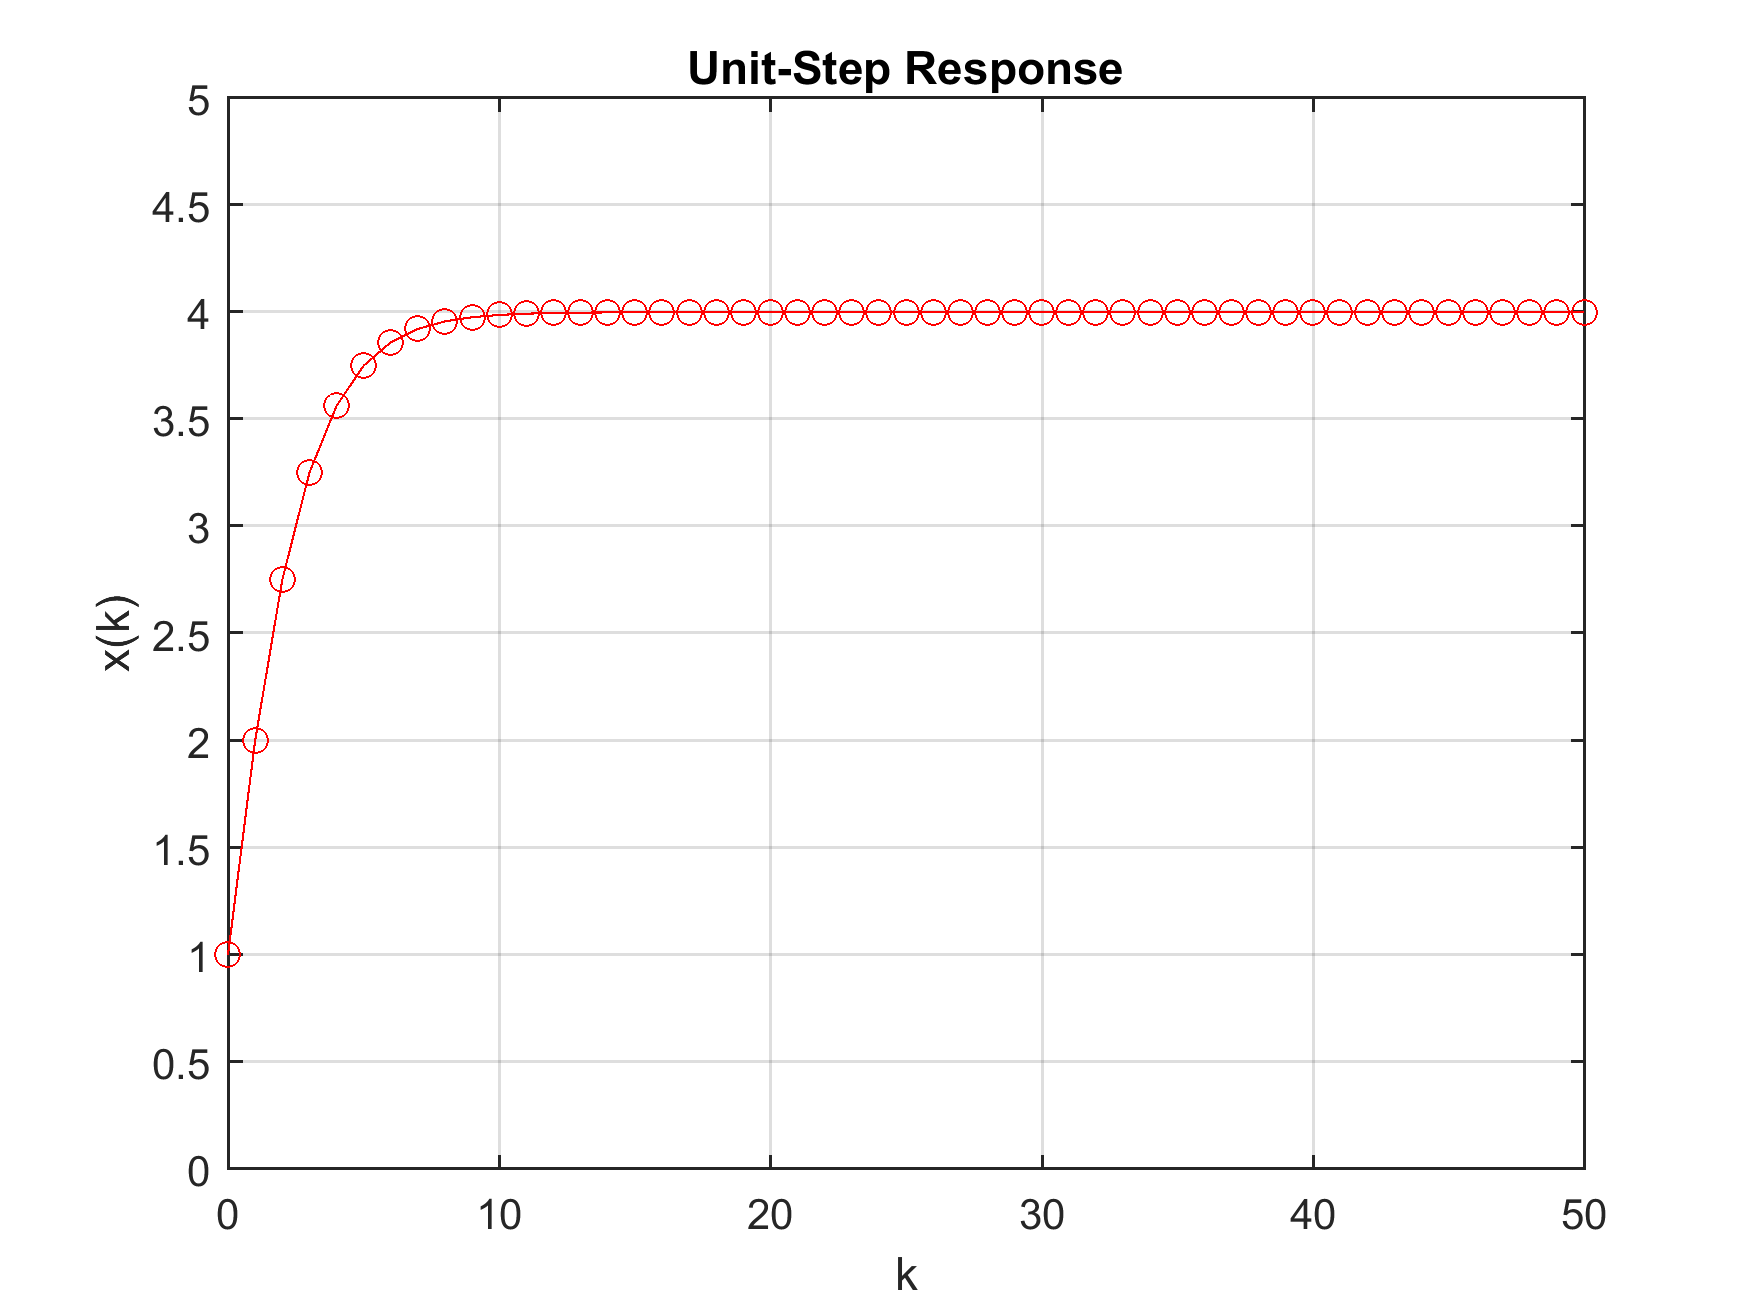
\includegraphics[width=1\linewidth]{B-2-17-matlab}
	\caption{Computational Approach to B-2-17 in Matlab}
	\label{fig:b-2-17-matlab}
\end{figure}

\nopagebreak
%4/(z - 1) - 4/(2*z - 1) - 1/(2*z - 1)^2 + 1